% Created 2021-01-24 Sun 22:49
% Intended LaTeX compiler: pdflatex
\documentclass[11pt]{article}
\usepackage[utf8]{inputenc}
\usepackage[T1]{fontenc}
\usepackage{graphicx}
\usepackage{grffile}
\usepackage{longtable}
\usepackage{wrapfig}
\usepackage{rotating}
\usepackage[normalem]{ulem}
\usepackage{amsmath}
\usepackage{textcomp}
\usepackage{amssymb}
\usepackage{capt-of}
\usepackage{hyperref}
\usepackage{minted}
\hypersetup{colorlinks=true, linkcolor=black, filecolor=red, urlcolor=blue}
\usepackage[turkish]{babel}
\author{Eren Hatırnaz}
\date{11 Mayıs 2020}
\title{Yazılım Gündemi - 2020/18\\\medskip
\large 4-10 Mayıs 2020}
\hypersetup{
 pdfauthor={Eren Hatırnaz},
 pdftitle={Yazılım Gündemi - 2020/18},
 pdfkeywords={},
 pdfsubject={},
 pdfcreator={Emacs 27.1 (Org mode 9.3)},
 pdflang={Turkish}}
\begin{document}

\maketitle
\tableofcontents \clearpage\shorthandoff{=}

\begin{center}
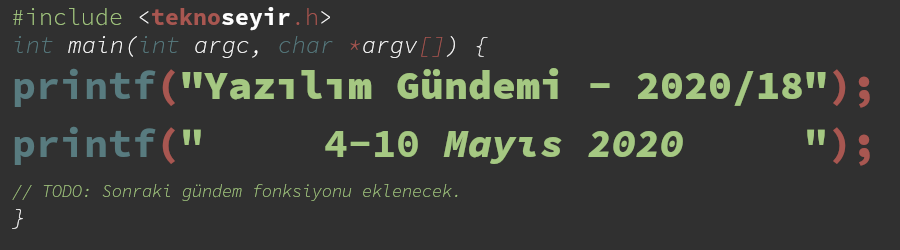
\includegraphics[width=.9\linewidth]{gorseller/yazilim-gundemi-banner.png}
\end{center}

\begin{center}
\href{../17/yazilim-gundemi-2020-17.pdf}{< Önceki Gündem} | \textbf{4-10 Mayıs 2020} | \href{../19/yazilim-gundemi-2020-19.pdf}{Sonraki Gündem >}

\href{https://teknoseyir.com/blog/yazilim-gundemi-2020-18}{TeknoSeyir'de Oku}
\end{center}

\section{GitHub, \href{https://githubsatellite.com/}{Satellite 2020} etkinliğini \href{https://github.blog/2020-05-06-new-from-satellite-2020-github-codespaces-github-discussions-securing-code-in-private-repositories-and-more/}{gerçekleştirdi}}
\label{sec:orgfcabb7e}
Geçtiğimiz yıllarda Microsoft tarafından satın alınan GitHub, geçtiğimiz hafta
içerisinde Satellite 2020 etkinliğini sanal olarak gerçekleştirdi. Etkinlikte
duyurulan yeniliklere birlikte göz atalım.

\subsection{GitHub Discussions}
\label{sec:org3c89b07}
\begin{figure}[htbp]
\centering
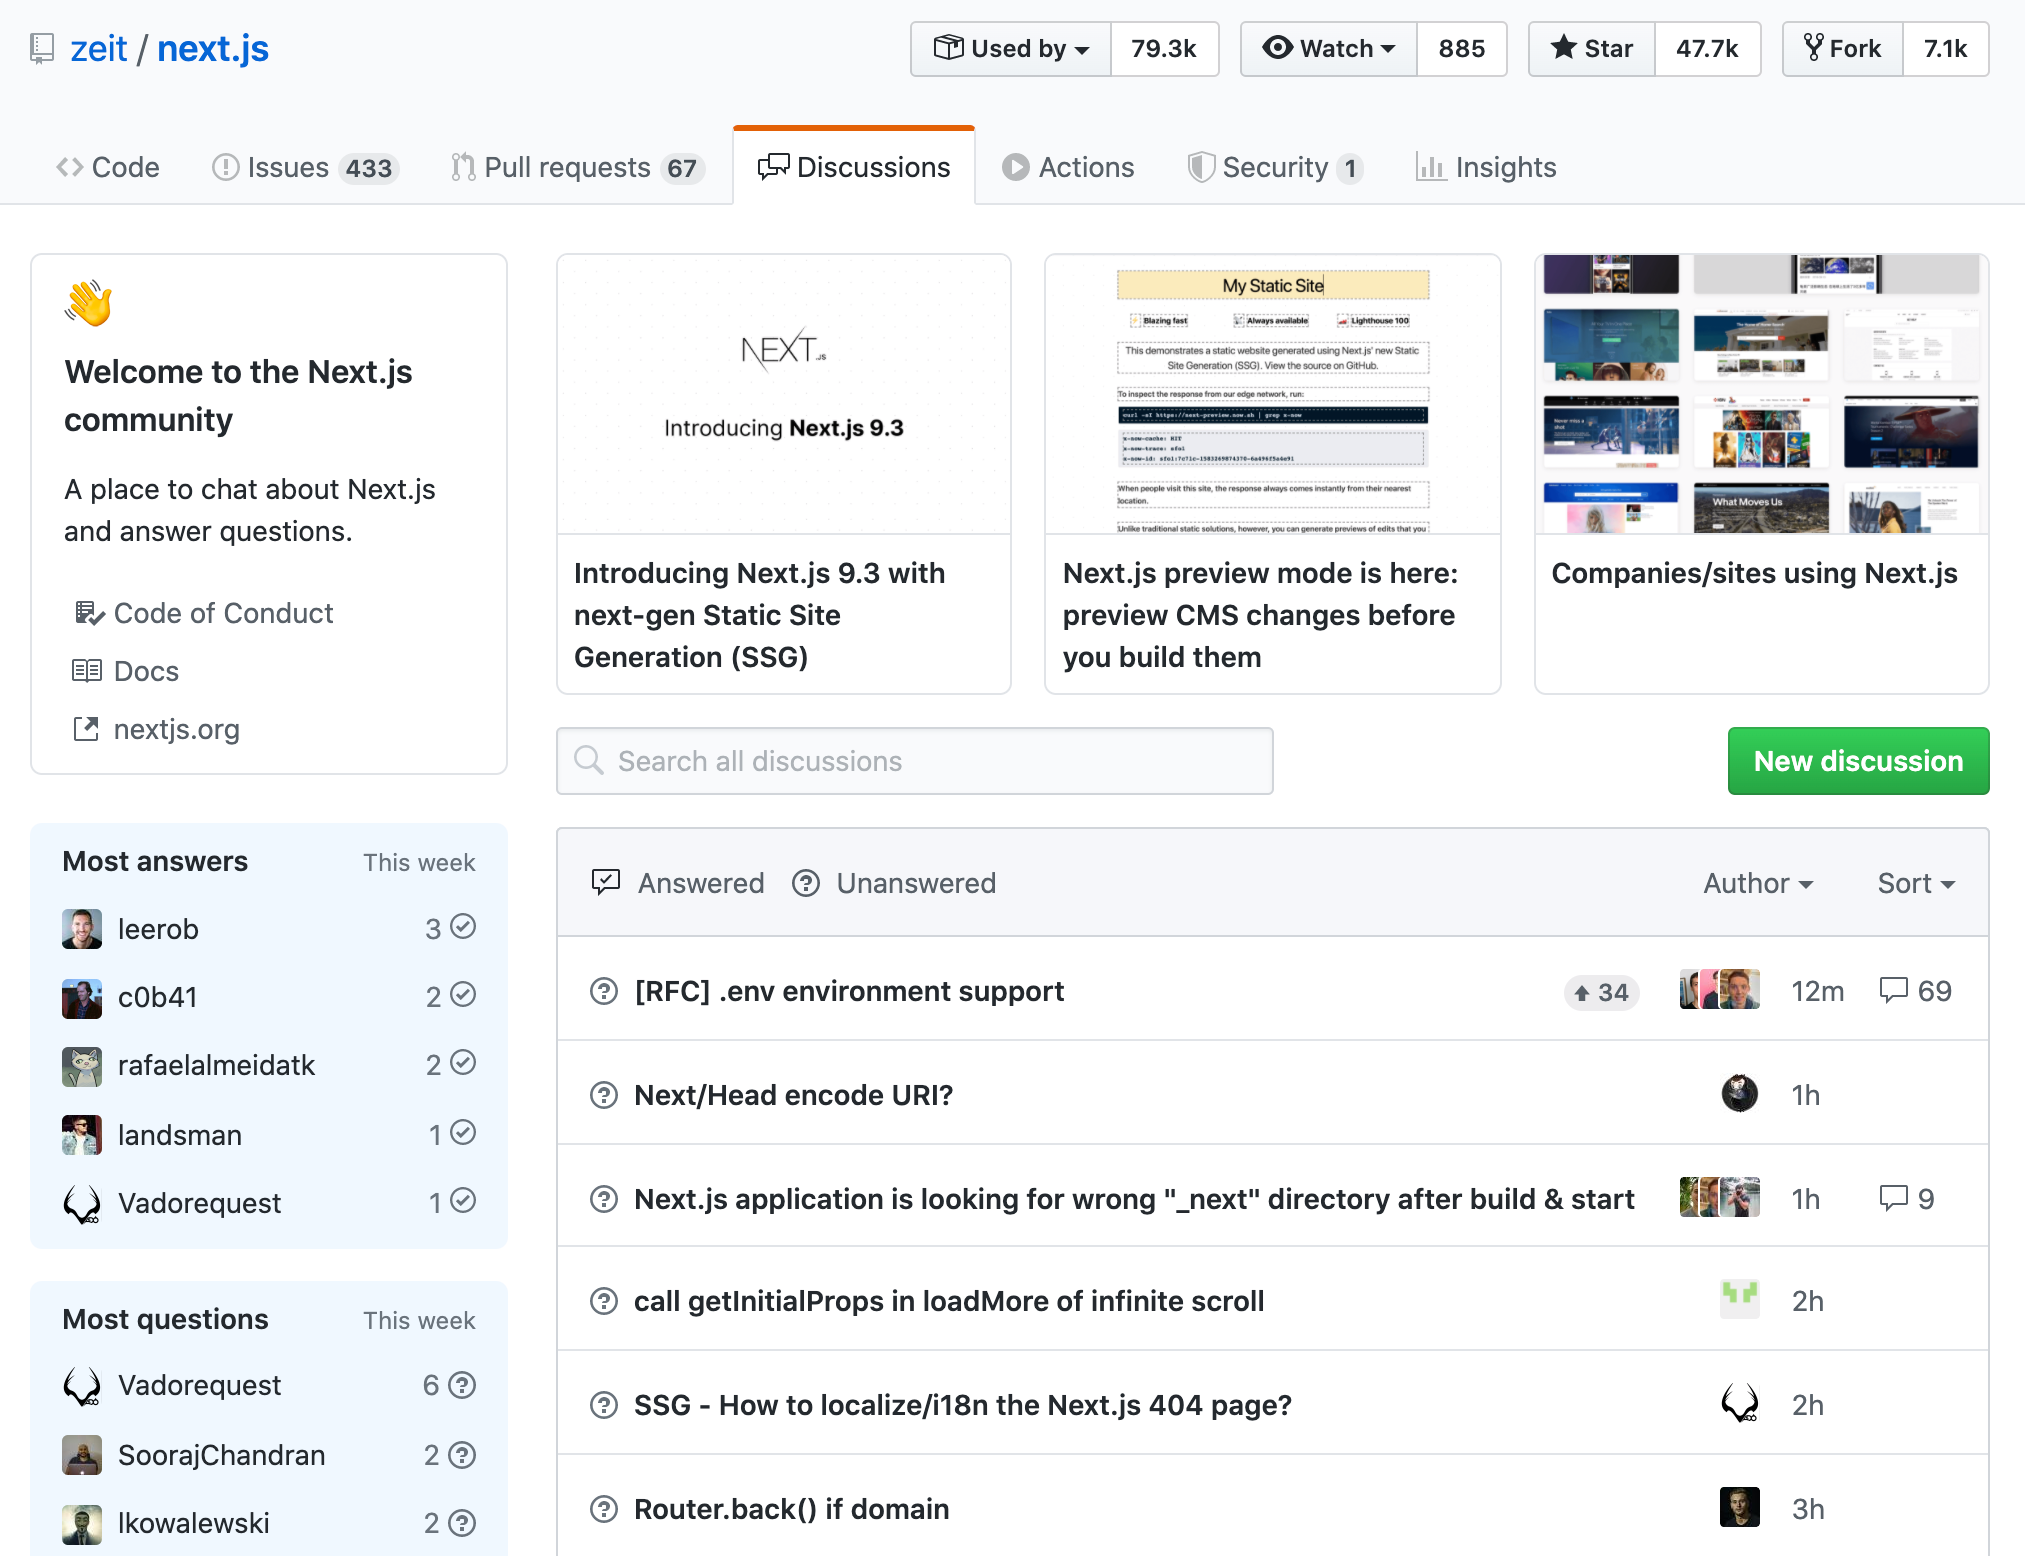
\includegraphics[height=6cm]{gorseller/github-discussions.png}
\caption[//github.com/zeit/next.js/discussions]{Örnek bir discussions sayfası için burayı ziyaret edebilirsiniz: \url{https://github.com/zeit/next.js/discussions}}
\end{figure}

Yazılım geliştiriciler olarak sıklıkla takıldığımız konularda yardım alma
ihtiyacımız oluyor. Uzun bir zamandır bu ihtiyacımızı StackOverflow üzerinde
gideriyorduk. Zaman zaman alternatifleri çıksa da StackOverflow kadar tutmadı
fakat artık yalnız değil. GitHub, Discussions özelliği ile doğrudan
StackOverflow'u hedef alıyor bence. Herkese açık depolar için yakında beta
olarak açılacak bu özellikle artık GitHub üzerinde proje sayfalarında da
ilgili projeyle ilgili sorular sorup, çözümü yazan kişilerin mesajlarını
çözüldü olarak işaretleyebileceğiz. Önceden beri issue sistemi zaten vardı
fakat bu discussions ile artık StackOverflow'daki gibi sorular sorabileceğiz.
GitHub ve StackOverflow arasında ortaya çıkan bu rekabet nereye varacak.
\subsection{\href{https://github.com/features/codespaces/}{GitHub Codespaces}}
\label{sec:orgf1170a0}
\begin{center}
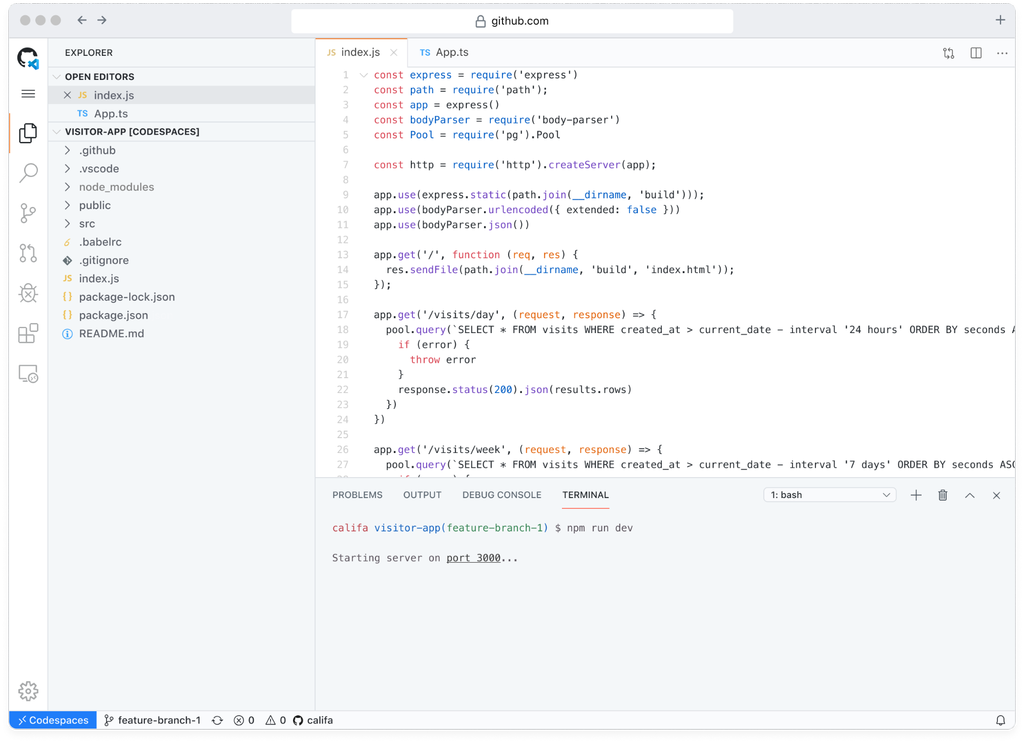
\includegraphics[height=6cm]{gorseller/github-codespaces.png}
\end{center}

Yazılım gündemi yazılarını takip edenler bu ismi mutlaka hatırlayacaklardır.
Evet, bir önceki gündem yazısından hatırlıyorsunuz. Microsoft, "Visual Studio
Online" olan cloud tabanlı geliştirme çözümünün ismini "Visual Studio
Codespaces" olarak değiştirmişti (bkz: \href{../17/yazilim-gundemi-2020-17.pdf}{Yazılım Gündemi - 2020/17}). Ne
tesadüftür ki bir başka Microsoft firması da aynı isimde özellik tanıtıyor
:). Çoğunuzun da anladığı üzere artık GitHub üzerinden tek bir tıklama ile
cloud tabanlı geliştirme ortamımızı ayağa kaldırabileceğiz. Henüz limitli
açık beta sürecinde ücretsiz olarak kullanılabilen bu özellik herkese
açıldığında kendine özel bir ücretlendirme ile gelecekmiş. Muhtemelen geçen
hafta duyurduğum "Visual Studio Codespaces"deki fiyatlarla aynı olacaktır.
GitHub'daki normal basit dosya düzenleme özelliği ücretsiz kalmaya devam
edecek tabii ki. Limitli açık beta için başvuru yapmıştım fakat henüz onay
gelmediği için detaylı bir şeyler yazamıyorum. Sizler de konu alt başlığına
tıklayarak özelliğin sunum sayfasına erişebilir, açık beta için başvuru
yapabilirsiniz. Onay alıp, deneme imkanınız olursa deneyimlerinizi yorumlar
bölümünde paylaşmaktan kendinizi geri koymayın.
\subsection{GitHub Codescanning ve Secret Scanning}
\label{sec:orgf433e4a}
Geçtiğimiz senenin yazılım gündemi yazılarının birinde (bkz: \href{../10/yazilim-gundemi-2020-10.pdf}{Yazılım
Gündemi - 10}) GitHub'ın Semmle isimli kod analizi çözümü sunan bir şirketi
satın aldığını haber yapmıştım ve "GitHub bunu mutlaka kullanır bir şekilde"
demiştim. İşte o kullanımlar geçtiğimiz hafta duyuruldu. Artık GitHub'a
yüklediğimiz kodlar üzerinde güvenlik açıkları ve zafiyetler için
otomatikleştirilmiş süreçler içeren 2 ürün var. Henüz ikisi de beta sürecinde
olsa da incelemeye değer.

\begin{center}
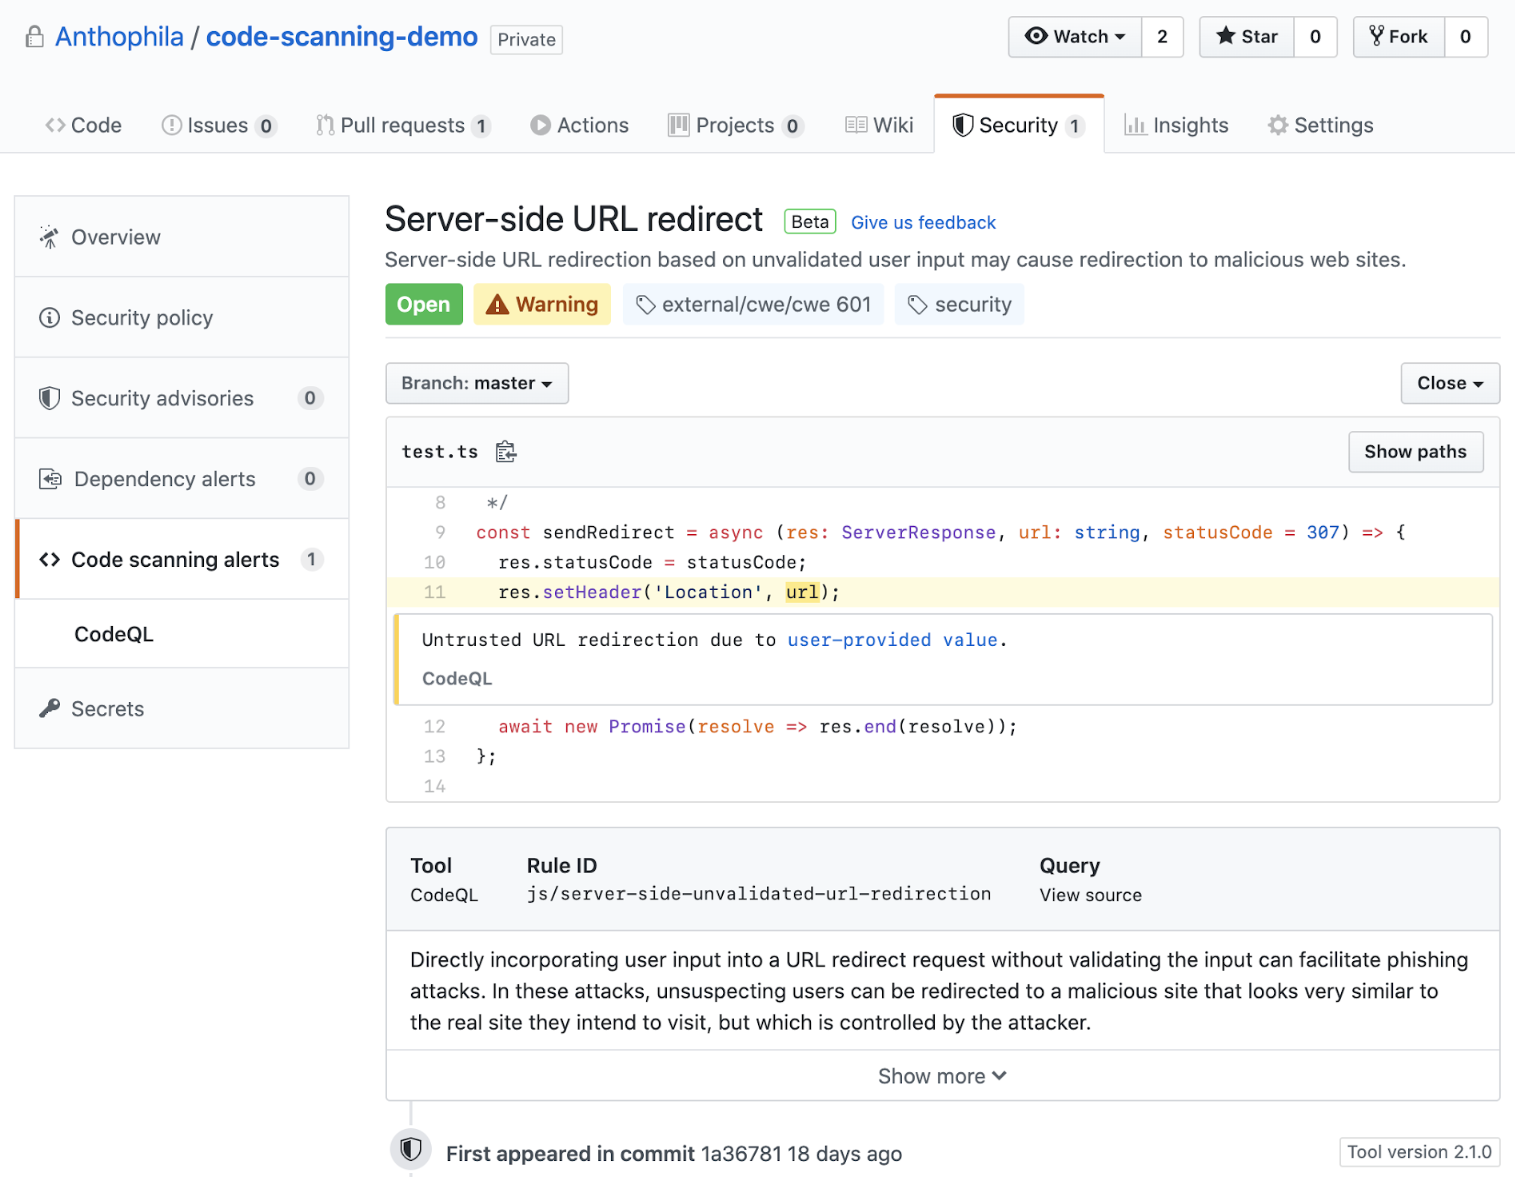
\includegraphics[height=6cm]{gorseller/github-codescanning.png}
\end{center}

\begin{itemize}
\item GitHub Code scanning ile herkese açık depolarımız üzerinde potansiyel
güvenlik açıklarına yönelik taramalar yapabiliyor ve bunu CI/CD gibi
süreçlerin bir parçası yapabiliyoruz. Yani "ben \texttt{git push} yaptığımda
otomatik olarak taramaları yap" diyebileceğiz. Olası güvenlik sorunlarına
karşı uyarı bildirimleri gönderen bu servis, arka planda GitHub tarafından
geliştirilen \href{https://github.com/github/codeql}{CodeQL} motorunu kullanıyor. Projeleriniz için beta
başvurusunda bulunmak için \href{https://github.com/features/security/advanced-security/signup}{bu sayfayı ziyaret edebilirsiniz}.
\item Secret scanning ise GitHub'da 2018'den beri olan bir özellik fakat artık
private depolarınız için de kullanabileceksiniz. Ne kadar dikkat etsek de
bazen boşta bulunup kodlar içerisinde olmaması gereken bir şifreyi ya da
gizli bir anahtarı unutabiliyoruz. Bu da haliyle güvenlik sorunlarına yol
açıyor. İşte secret scanning tam da bu sorunu çözmeye yönelik bir özellik.
Projelerinizde şifreye ya da gizli anahtara benzer metinsel ifadeler
gördüğünde sizi uyarıyor ve yapmanız gerekenler hakkında bilgi veriyor.
\end{itemize}


GitHub'ın bu mecburiyetten dolayı sanal olarak düzenlediği Satellite 2020
etkinliğinde duyurulan belli başlı özellikler bu şekildeydi. Etkinliğin toplam
12 saatlik kaydı YouTube üzerinde mevcut, \href{https://www.youtube.com/watch?v=FhZTPM9ysWk\&feature=emb\_title}{buraya tıklayarak ilgili videoya
erişebilirsiniz}.

Gördüğünüz gibi GitHub yazılım geliştirme ekosisteminin her alanı için bir
çözüm üretmeye devam ediyor. Elbette çoğu geliştirici için GitHub'da tüm
işlerini halledebilmek çok büyük bir kolaylık olacaktır ama ben GitHub'ın
sektördeki konumundan da dolayı giderek tekelleştiğini düşünmeye başladım.
Elbette bir firma açısından baktığımızda müşterilerini başka firmaların
ürünlerini kullanmak zorunda bırakmadan, kendi bünyesi içerisinden çözümler
sunmak istemesi çok doğal fakat ben şahsen yazılım geliştirmeyle ilgili her
şeyimi GitHub'a emanet etmek istemezdim. Bunun için de haklı nedenlerim
olduğunu düşünüyorum. Geçmişte Amerika'nın ambargo uyguladığı ülkelerdeki
geliştiricilerin hesaplarını nasıl kilitlediklerini ve kodlarına resmen el
koyduklarını hep birlikte görmüştük (bkz: \href{../../2019/03/yazilim-gundemi-03.pdf}{Yazılım Gündemi - 3}). Elbette tüm
kararınızı olası bir "ambargo" kararına göre vermek mantıklı değil fakat
Levent Abi'nin sözünü tekrar hatırlatmak istiyorum: "/Cloud dediğin başkasının
bilgisayarıdır. Gün gelir de 'sana hizmet vermiyorum kardeşim' derse
yapabileceğin bir şey yok/". Bu konuda siz ne düşünüyorsunuz? GitHub'ın bu
kadar büyümesi ve yeni hizmetler sağlaması sizi endişelendiriyor mu? Yoksa bu
yönde çekinceleriniz yok mu? Yorumlar bölümünde konuşalım.
\section{Microsoft'un GitHub \href{https://www.bleepingcomputer.com/news/security/microsofts-github-account-hacked-private-repositories-stolen/}{hesabı hacklendi}}
\label{sec:orgce755cb}
\href{https://www.bleepingcomputer.com/}{BleepingComputer} sitesinin geçtiğimiz hafta yayınladığı habere göre "Shiny
Hunter" rumuzlu hacker, Microsoft çalışanlarından birinin GitHub hesabını
hackleyerek, private (herkese açık olmayan) depolara erişim sağladığını ve
500GB'dan daha fazla büyüklükte veri çaldığını iddia etti. Haftanın ilerleyen
günlerinde ise bir Microsoft çalışanından olayın gerçek olduğunu öğrendik.

\begin{figure}[htbp]
\centering
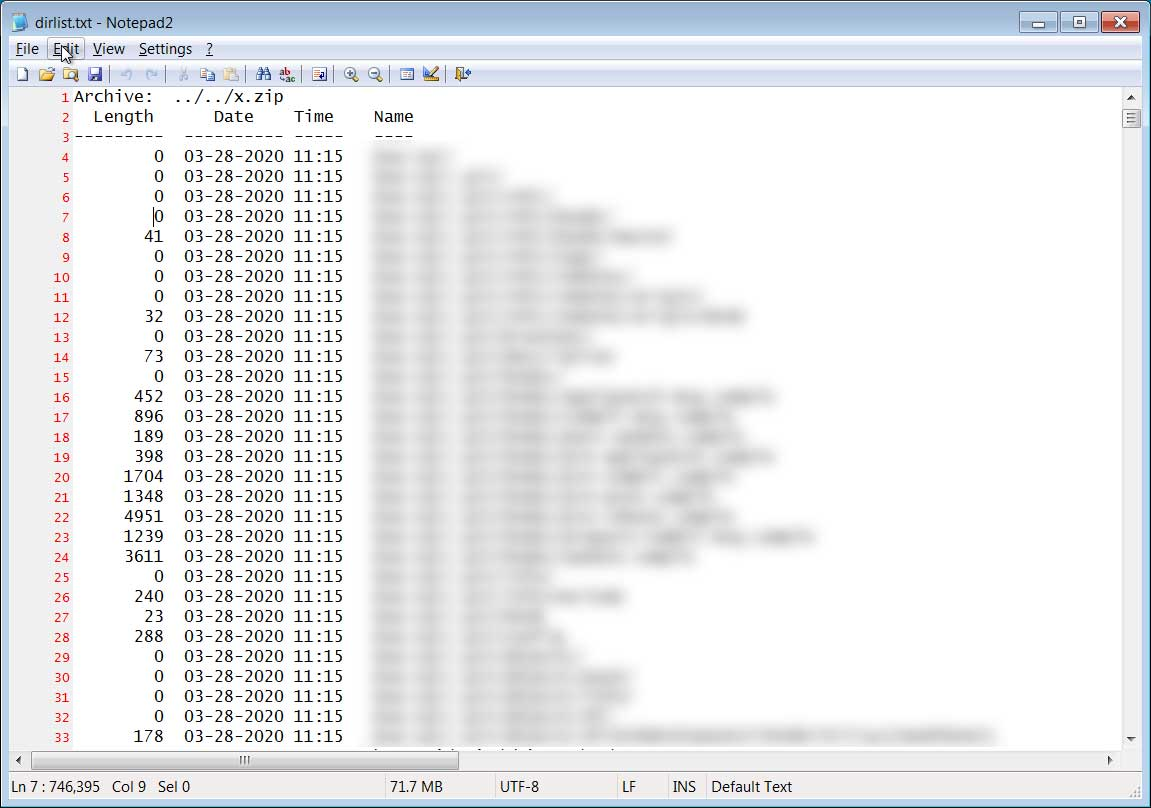
\includegraphics[height=6cm]{gorseller/microsoft-github-leak.jpg}
\caption{Hacker'ın paylaştığı ekran görüntüsündeki tarih bilgilerinden olayın 28 Mart günü gerçekleştiği ortaya çıkıyor.}
\end{figure}

Hacker ilk bu verileri yer altı forumlarında satmayı düşünmüş olsa da,
sonradan ücretsiz olarak sızdırmayı tercih etmiş gibi gözüküyor.
BleepingComputer sitesinin incelediğine göre sıvan private repoların içinde
Microsoft'u zora sokacak derecede projelerin kodları yok. Çoğunlukla gizlilik
gerektirmeyen kodlar, kod örnekleri, test projeleri ve e-kitapların yer aldığı
söyleniyor. Zaten bu yüzden de pek fazla ses getirmedi bu olay ve çok az
konuşuldu.
\section{Facebook SDK kütüphanesindeki bir hata, popüler iOS uygulamalarının \href{https://www.theverge.com/2020/5/7/21250689/facebook-sdk-bug-ios-app-crash-apple-spotify-venmo-tiktok-tinder}{çökmesine yol açtı}}
\label{sec:org6ff6f4d}
Günümüzde birçok mobil uygulama ve web sitenin açılış ekranlarında çok sık
"Facebook ile giriş yap", "Twitter ile kayıt ol" tarzı alternatif kimlik
doğrulama yöntemlerini görüyoruz. Biz yazılım geliştiriciler olarak bu tarz
özellikleri yine ilgili sosyal medya sitesinin sağladığı Software Development
Kit'ler (SDK) aracılığıyla uygulamalarımıza ya da web sitelerimiz ekliyoruz.
Geçtiğimiz hafta içerisinde de Facebook'un sağladığı SDK paketinin iOS
sürümünde çıkan bir hata, bu paketi kullanan popüler iOS uygulamalarının
açılırken çökmesine yol açtı. Bu uygulamalar arasında Spotify, TikTok ve
Pinterest gibi uygulamalar da var. "Facebook ile giriş yap" özelliğinden
faydalanmayan kullanıcılar da durumdan etkilenmişler.

\begin{itemize}
\item \href{https://twitter.com/aburninghilll/status/1258169688959352832}{Konuyla ilgili Tweet}
\end{itemize}

Olay hakkında daha detaylı bilgi için konu başlığına eklediğim bağlantıya
tıklayabilirsiniz ya da Facebook'un iOS SDK paketinin GitHub deposundaki \href{https://github.com/facebook/facebook-ios-sdk/issues/1374}{şu
issue sayfasını} ziyaret edebilirsiniz. Uygulama geliştiren arkadaşların
Facebook SDK ile olan bağlarını tekrar gözden geçirmelerini tavsiye ederim.
\section{\href{https://medium.com/flutter/announcing-flutter-1-17-4182d8af7f8e}{Flutter 1.17} ve \href{https://medium.com/dartlang/announcing-dart-2-8-7750918db0a}{Dart 2.8} sürümleri yayınlandı}
\label{sec:org46d2592}
Google tarafından geliştirilen platformlar-arası (cross-platform) uygulama
geliştirme framework'ü Flutter ve programlama dili Dart, geçtiğimiz hafta
içerisinde yeni sürümlerini yayınladılar. Birbiriyle ilişkili iki teknoloji
olduğu için birlikte değerlendirmek istedim.

Flutter 1.17 ile birlikte gelen bazı yenilik ve değişiklikler:
\begin{itemize}
\item \textbf{Mobil performans ve boyut iyileştirmeleri}: Hiçbir şey yapmadan sadece
uygulamanızın Flutter sürümünü 1.17'ye yükselterek bile daha hızlı
animasyonlar, daha küçük uygulama boyutları ve daha az bellek kullanımları
elde edebiliyorsunuz. Flutter takımının iddiasına göre \%40 oranında CPU/GPU
kullanımında azalma ve uygulama boyutunda \%18.5'lik bir azalma oluyor.
Flutter'ın örnek \href{https://github.com/flutter/gallery}{Flutter Galery} uygulaması bu sürüm değişikliğiyle birlikte
9.6MB'dan 8.1MB'a düşmüş.
\item \textbf{iOS için Metal desteği, \%50'lik bir performans iyileştirmesi sağlıyor}:
OpenGL gibi bir grafik kütüphanesi olan ve Apple tarafından geliştirilen
Metal, artık Flutter'ın iOS tarafında varsayılan olarak kullandığı grafik
kütüphanesi haline gelmiş. Apple tarafından geliştirilmesinden dolayı da iOS
işletim sisteminde iyi performansla çalışabiliyor. Artık Flutter ile
geliştirdiğimiz uygulamaların grafik işlemleri öncekine göre daha hızlı
gerçekleşecek.
\item \textbf{Material tasarıma sahip yeni widget'lar}: \texttt{NavigationRail}, \texttt{DatePicker}.
Doğrudan Google Material Design takımı tarafından tasarlanan bu yeni
widget'lar artık Flutter 1.17 ile emrinize amade.

\url{gorseller/flutter1-17-navigationrail.gif}

\url{gorseller/flutter1-17-datepicker.gif}
\end{itemize}

Dart programlama dili kendi içerisinde \texttt{pub} isimli bir paket yöneticisi
(bağımlılık yöneticisi) ile birlikte geliyor. Geçtiğimiz hafta yayınlanan Dart
2.8 sürümüyle de Dart takımının bu paket yöneticisini daha iyileştirmeye
yönelik çalışmalar yaptığını görebiliyoruz. Şöyle ki:
\begin{itemize}
\item * \texttt{pub get} komutunda hız iyileştirmeleri*: Artık \href{https://pub.dev/}{pub.dev} üzerinden
paketleri daha hızlı indirebileceğiz. Flutter takımı örnek veri olarak
Flutter 1.12 sürümünde \texttt{flutter create} komutunun 6.5 saniye sürdüğünü,
fakat artık Dart 2.8'de bunun sadece 2.5 saniye sürdüğünü belirtmiş.
\item *Yeni komut \texttt{=pub outdated} *: Bu yeni komut sayesinde artık eski sürümde
kalmış kütüphaneleri daha kolay tespit edebilecek ve sürümler arası
geçişler için daha fazla bilgi edinebileceksiniz.
\end{itemize}

Flutter 1.17 ve Dart 2.8 ile birlikte gelen diğer özellik ve değişiklikler
için konu başlığına eklediğim bağlantılara tıklayabilirsiniz.
\section{Firefox 76 ile \href{https://hacks.mozilla.org/2020/05/firefox-76-audio-worklets-and-other-tricks/}{gelen yeni özellikler}}
\label{sec:org2ca2c3a}
Popüler web tarayıcılardan biri olan Mozilla Firefox, geçtiğimiz hafta
içerisinde 76.0 numaralı sürümünü yayınladı. Bu sürümle birlikte gelen ve biz
geliştiricileri ilgilendiren yeni özelliklerin birkaçına birlikte bakalım.

\subsection{Debug yaparken dizini tamamen görmezden gelme}
\label{sec:org8136b01}
Her ne kadar çoğumuz hata ayıklama (debug) için \texttt{printf}, \texttt{echo},
\texttt{console.log} gibi komutları kullansak da tarayıcıların sağladığı Debugger
özelliği bazı durumlarda daha işe yarar olabiliyor. Bu durumlarda da
genellikle sadece proje klasörünüzün içerisindeki dosyaları debug etmek,
oradaki olaylara bakmak isterseniz. İşte Firefox 76 ile birlikte gelen
"\emph{blackboxing}" özelliği ile bu mümkün. \textbf{\textbf{Debugger}} panelinin, \textbf{\textbf{Sources}}
sekmesinden bir dizin seçip "\emph{bu dizin içindeki tüm dosyaları görmezden gel
(ignore)}" ya da "\emph{bu dizin haricindeki tüm dizinleri görmezden gel}"
diyebileceğiz.

\url{gorseller/firefox76-dizin-gormezden-gel.gif}
\subsection{\href{https://developer.mozilla.org/en-US/docs/Web/API/Web\_Audio\_API/Using\_AudioWorklet}{Audio Worklets}}
\label{sec:org7f9323a}
Firefox 76 ile birlikte gelen bu yeni API sayesinde tarayıcı üzerinde arka
planda ses işleme süreçleri işletebileceğiz. Açıkcası benim de çok yabancı
olduğum bir alan fakat ilgili arkadaşlar alt konu başlığına eklediğim
bağlantıya tıklayarak detaylı dokümantasyon yazısına ulaşabilirler.
\subsection{Developer Edition için: CSS Uyumluluk Paneli}
\label{sec:orgc84809a}
Bildiğiniz gibi Mozilla, Firefox'un bir de pre-release kanalı olarak
Developer Edition sürümünü kullanıma sürüyor. Bu sürümde genelde sonraki
Firefox sürümlerinde olan özellikler önceden geliştiricilerin kullanımına
açılıyor ve test ediliyor. Bu özelliklere bir yenisi daha eklendi. F12 ile
açtığımız Geliştirici Araçlarındaki CSS bölümüne artık \textbf{Compatibility}
sekmesi de eklendi. Bu sekme sayesinde seçilen HTML elamanındaki aktif CSS
özelliklerinin hangi tarayıcılarda desteklendiğini görebiliyoruz.

\begin{center}
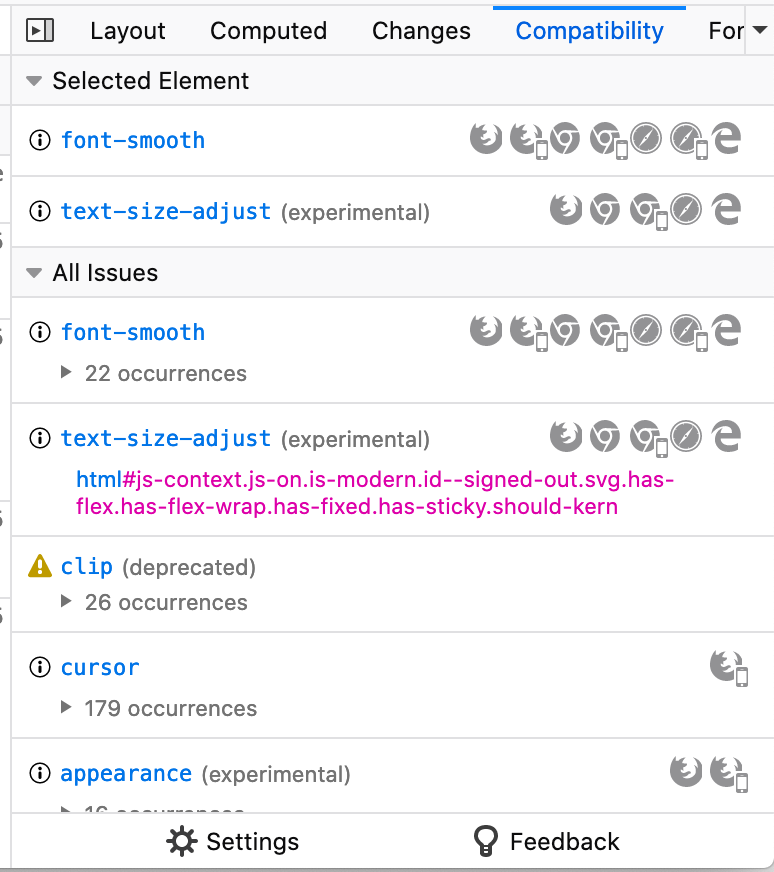
\includegraphics[height=5.7cm]{gorseller/firefox76-css-uyumluluk-panel.png}
\end{center}

Firefox 76 ile birlikte gelen diğer geliştirici özellikleri için konu
başlığına eklediğim bağlantıya tıklayabilirsiniz.
\section{TIOBE popüler programlama dilleri sıralamasını \href{https://jaxenter.com/c-programming-may-2020-171598.html}{Mayıs 2020 için güncelledi}}
\label{sec:orgff66bd8}
Belirli periyotlarla internetteki programlama trendlerini analiz edip
bunlardan programlama dilleri popülerliğini çıkartan TIOBE firması, Mayıs 2020
için güncel popüler programlama dilleri sıralamasını geçtiğimiz hafta
içerisinde yayınlandı. Yeni tablo bu şekilde:

\begin{center}
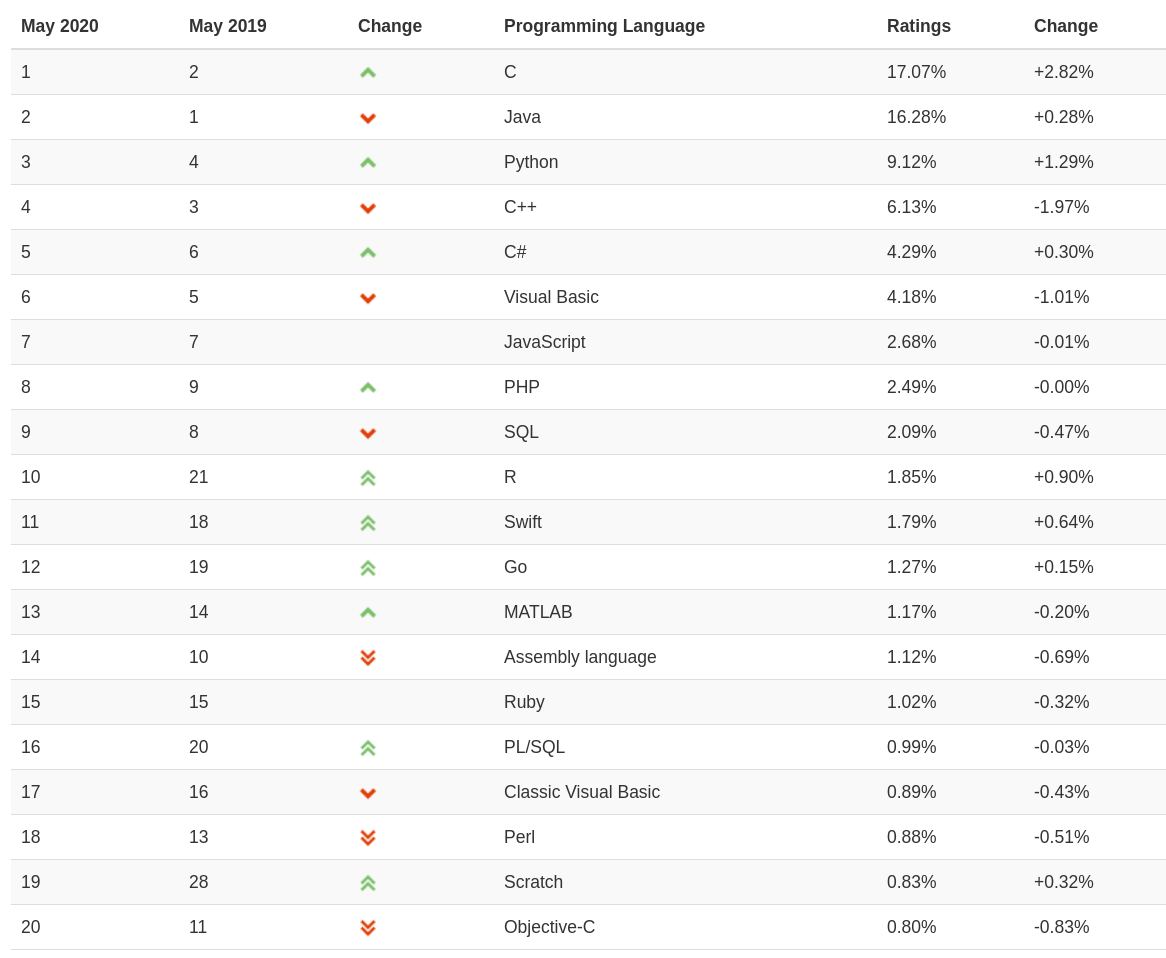
\includegraphics[height=6.5cm]{gorseller/tiobe-index.png}
\end{center}

Elbette bu liste sadece popülerliğe göre belirlendiği için bizim için çok bir
anlam ifade etmiyor. Sonuçta geliştireceğimiz yazılımlarda işimize en uygun
olanı hangisiyse onu tercih ediyoruz, popülerlik sıralamasına göre tercih
yapmıyoruz ama yine de programlama alanıyla ilgili olduğu için gündeme almak
istedim.

Daha detaylı analizler ve interaktif grafikler için TIOBE sitesindeki \href{https://www.tiobe.com/tiobe-index/}{bu
sayfayı} ziyaret edebilirsiniz.
\section{Visual Studio Code \href{https://code.visualstudio.com/updates/v1\_45}{Nisan 2020 (v1.45) sürümü yayınlandı}}
\label{sec:org2eb3e0c}
\begin{center}
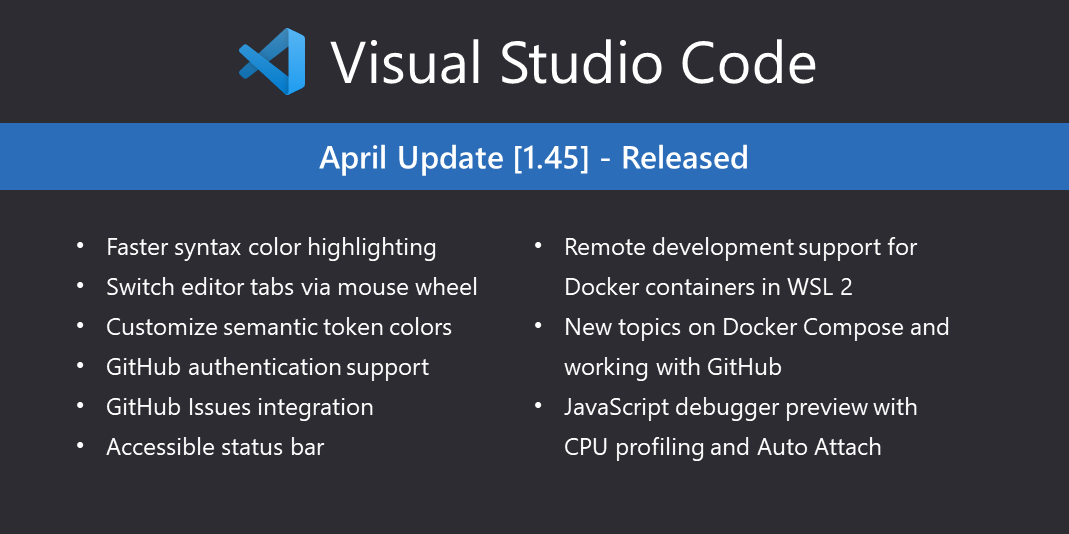
\includegraphics[width=.9\linewidth]{gorseller/vscode1-45.png}
\end{center}
\section{Yaklaşan Online Etkinlikler \#EvdeKal}
\label{sec:org357459d}
\begin{longtable}{|p{9.5cm}|l|}
\hline
Etkinlik İsmi & Tarihi\\
\hline
\endfirsthead
\multicolumn{2}{l}{Önceki sayfadan devam ediyor} \\
\hline

Etkinlik İsmi & Tarihi \\

\hline
\endhead
\hline\multicolumn{2}{r}{Devamı sonraki sayfada} \\
\endfoot
\endlastfoot
\hline
\href{https://kommunity.com/tracikkaynak/events/acik-seminer-18-gun-olceklenebilir-makine-ogrenimi-uygulamalari-621dca47}{Açık Seminer 18. Gün: Ölçeklenebilir Makine Öğrenimi Uygulamaları} & 12 Mayıs 14:00\\
\href{https://kommunity.com/cozumpark/events/uzaktan-siber-guvenlik-yaklasimi-ve-olaylari-monitor-etme-c989475b}{Uzaktan Siber Güvenlik Yaklaşımı ve Olayları Monitör Etme} & 12 Mayıs 14:00\\
\href{https://kommunity.com/akademi/events/malware-forensics-zararli-yazilim-tespiti-webinar-dc4a41a9}{Malware Forensics - Zararlı Yazılım Tespiti} & 12 Mayıs 16:30\\
\href{https://kommunity.com/cloud-and-serverless-turkey/events/ramazan-ozel-6-devops-vs-sre-41220ba0}{DevOps vs SRE} & 12 Mayıs 23:00\\
\href{https://kommunity.com/cozumpark/events/siber-guvenlikte-tehdit-avciligi-threat-hunting-21ee4d23}{Siber Güvenlikte Tehdit Avcılığı (Threat Hunting)} & 13 Mayıs 14:00\\
\href{https://kommunity.com/tracikkaynak/events/acik-seminer-19-gun-watson-apis-chatbot-and-vr-implementations-68e687f7}{Açık Seminer 19. Gün: Watson APIs, Chatbot and VR Implementations} & 13 Mayıs 14:00\\
\href{https://kommunity.com/mavidurakio/events/s1e41-yazilimci-bulusmasi-52fe964f}{Yazılımcı Buluşması \{MaviDurak-IO\}} & 13 Mayıs 21:15\\
\href{https://kommunity.com/bilge-adam-teknoloji/events/nodejs-ile-uygulama-gelistirme-d4055b37}{Node.js ile Uygulama Geliştirme} & 13 Mayıs 21:15\\
\href{https://kommunity.com/devops-turkiye/events/aws-suspicious-activity-monitoring-with-humio-f70d68e0}{AWS suspicious activity monitoring with humio} & 13 Mayıs 22:00\\
\href{https://kommunity.com/tracikkaynak/events/acik-seminer-20-gun-microsoft-yapay-zeka-servislerine-genel-bakis-2a911429}{Açık Seminer 20. Gün: Microsoft Yapay Zeka Servislerine Genel Bakış} & 14 Mayıs 14:00\\
\href{https://kommunity.com/dotnet-istanbul/events/net-core-ile-restful-api-design-fe171c15}{.NET Core ile RESTful API Design} & 15 Mayıs 22:00\\
\href{https://kommunity.com/cloud-and-serverless-turkey/events/ramazan-ozel-7-faas-serverless-aws-lambda-problemleri-ve-cozumleri-5888dd48}{FaaS - Serverless (AWS Lambda) Problemleri ve Çözümleri} & 15 Mayıs 23:00\\
\href{https://kommunity.com/cloud-and-serverless-turkey/events/kubernetes-hands-on-3-volume-and-configuration-management-2547c2f3}{Kubernetes Hands-On no.3: Volume And Configuration Management} & 17 Mayıs 13:30\\
\hline
\end{longtable}
\section{Diğer Haberler}
\label{sec:orgcdf034e}
\begin{itemize}
\item İngiltere, COVID-19 takibi için geliştirdiği mobil uygulamaların kodlarını
\href{https://github.com/nhsx}{açık kaynak hale getirdi}.
\item Avustralya, COVIDSafe uygulamasının kodlarını \href{https://www.dta.gov.au/news/dta-publicly-releases-covidsafe-application-source-code}{açık kaynak hale getirdi}.
\item GitHub, Covid-19 süresinde geliştiricilerin üretkenlikleriyle ilgili bir
\href{https://github.blog/2020-05-06-octoverse-spotlight-an-analysis-of-developer-productivity-work-cadence-and-collaboration-in-the-early-days-of-covid-19/}{analiz raporu yayınladı}.
\item Microsoft, Yapay Zeka ile ilgilenenler için yeni \href{https://www.zdnet.com/article/microsoft-our-new-free-python-programming-language-courses-are-for-novice-ai-developers/}{Python eğitim serisini
duyurdu}.
\item Microsoft, Yeni Zelanda'da veri merkezi kurmayı \href{https://news.microsoft.com/en-nz/2020/05/06/aotearoa-disclosure/}{planladığını açıkladı}.
\item AWS, EC2 hizmetinin fiyatlarını \href{https://aws.amazon.com/blogs/aws/ec2-price-reduction-for-ec2-instance-saving-plans-and-standard-reserved-instances/}{düşürdüğünü açıkladı}.
\item Backblaze, B2 Bulut Depolama çözümünün artık AWS S3 API'leri ile \href{https://www.backblaze.com/blog/backblaze-b2-s3-compatible-api/}{uyumlu
olduğunu duyurdu}.
\item GCC \href{https://gcc.gnu.org/pipermail/gcc-announce/2020/000163.html}{10.1 sürümü yayınlandı}. \href{https://gcc.gnu.org/gcc-10/changes.html}{Detaylı Yazı}
\item Unreal Engine \href{https://www.unrealengine.com/en-US/blog/unreal-engine-4-25-released}{4.25 sürümü yayınlandı}.
\item Rust programlama dilinin \href{https://blog.rust-lang.org/2020/05/07/Rust.1.43.1.html}{1.43.1 sürümü yayınlandı}.
\item Racket programlama dilinin \href{https://download.racket-lang.org/v7.7.html}{v7.7 sürümü yayınlandı}.
\item Bolt programlama dilinin \href{https://github.com/mukul-rathi/bolt/releases/tag/1.0}{1.0 sürümü yayınlandı}.
\item Anvil, Runtime Engine aracını \href{https://anvil.works/blog/open-source}{açık kaynak hale getirdi}. \href{https://github.com/anvil-works/anvil-runtime}{GitHub Deposu}
\item Merkesizleştirilmiş uygulama geliştirme ve ölçekleme için \href{https://blog.textile.io/announcing-the-textile-protocol-hub/}{yeni bir araç
kutusu duyuruldu}: Textile Hub.
\item Go ile yazılmış web sunucusu Caddy'nin \href{https://github.com/caddyserver/caddy/releases/tag/v2.0.0}{v2.0.0 sürümü yayınlandı}.
\item TileDB \href{https://medium.com/tiledb/tiledb-2-0-and-the-future-of-data-science-929cdcfe95ed}{2.0 sürümü yayınlandı}.
\item Beekeeper Studio \href{https://www.beekeeperstudio.io/blog/release-1.2}{v1.2 sürümü yayınlandı}.
\item Lite metin editörünün \href{https://github.com/rxi/lite/releases/tag/v1.03}{1.03 sürümü yayınlandı}.
\item C++ oyun kütüphanesi EnTT \href{https://github.com/skypjack/entt/releases/tag/v3.4.0}{3.4.0 sürümü yayınlandı}.
\item Kubernetes IDE'si Lens, \href{https://github.com/lensapp/lens/releases}{v3.4.0 sürümünü yayınladı}.
\item Platformlar-arası terminal arayüzü kütüphanesi LTUI \href{https://github.com/tboox/ltui/wiki/LTUI-v1.7-released,-A-cross-platform-terminal-ui-library-based-on-Lua}{v1.7 sürümünü yayınladı}.
\item OpenAPIGenerator \href{https://mobile.twitter.com/oas\_generator/status/1258057660974329861}{v7.7 sürümü yayınlandı}.
\item StellarGraph \href{https://medium.com/stellargraph/stellargraph-1-0-taking-graph-machine-learning-to-a-new-level-2bd6a04fbc77}{1.0 sürümü yayınlandı}.
\end{itemize}
\section{Lisans}
\label{sec:org921ba9e}
\begin{center}
\begin{center}

\includegraphics[height=1.5cm]{../../../img/CC_BY-NC-SA_4.0.png}
\end{center}

\href{yazilim-gundemi-2020-18.pdf}{Yazılım Gündemi - 2020/18} yazısı \href{https://erenhatirnaz.github.io}{Eren Hatırnaz} tarafından \href{http://creativecommons.org/licenses/by-nc-sa/4.0/}{Creative Commons
Atıf-GayriTicari-AynıLisanslaPaylaş 4.0 Uluslararası Lisansı} (CC BY-NC-SA 4.0)
ile lisanslanmıştır.
\end{center}
\end{document}
